
\section{Sigma-Delta-ADC}

\subsection{Aufbau Sigma-Delta-ADC}
\label{Aufbau Sigma-Delta-ADC}

\begin{minipage}[t]{0.6\columnwidth}
    \begin{center}
        \myul{Sigma-Delta-ADC}
    \end{center}
    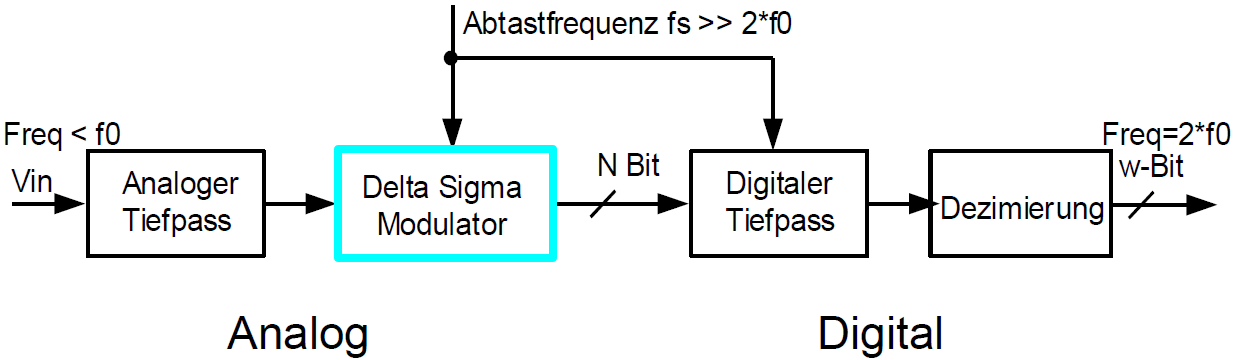
\includegraphics[width=\columnwidth]{images/aufbau_sigma_delta_ADC.png}
\end{minipage}
\hfill
\begin{minipage}[t]{0.38\columnwidth}
    \begin{center}
        \myul{Detail: Sigma-Delta-Modulator}
    \end{center}
    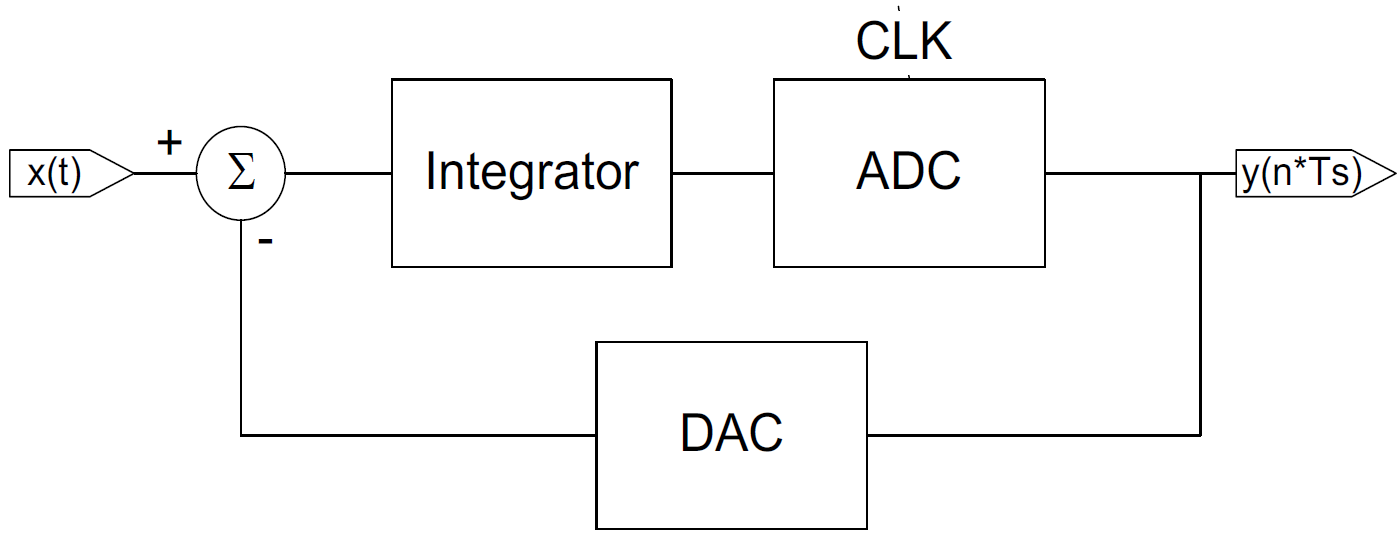
\includegraphics[width=\columnwidth]{images/aufbau_sigma_delta_modulator.png}
\end{minipage}


\subsection{Sigma-Delta-Modulator 1. Ordnung}
\label{Sigma-Delta-modulator Ordnung 1}

\begin{minipage}[c]{0.48\columnwidth}
    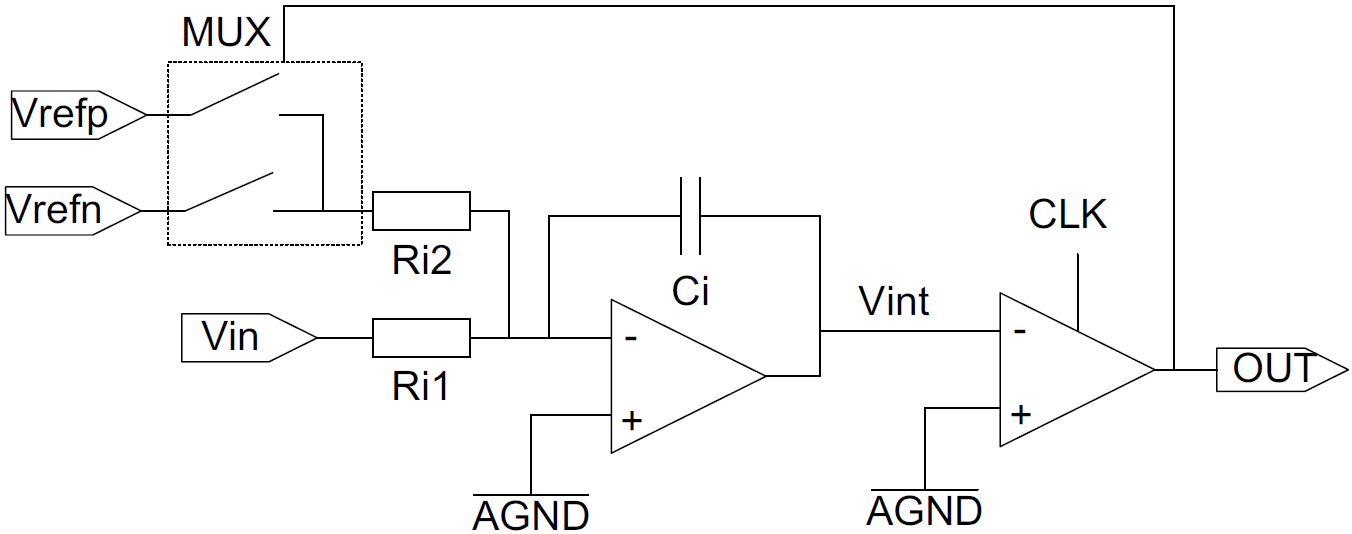
\includegraphics[width=\columnwidth]{images/sigma-delta-wandler.png}
\end{minipage}
\hfill
\begin{minipage}[c]{0.48\columnwidth}
    $$ \boxed{V_{\rm in} = \frac{2 \cdot n  - N}{N} V_{\rm ref}} $$

    \begin{tabular}{ll}
        $N$ & \# Taktzyklen von Clk \\
        $n$ & \# Taktzyklen, in denen \\
            & Modulator-Ausgang $=1$
    \end{tabular}
\end{minipage}
$$\boxed{\text{Allgemein: } V_{\rm int}(t) = \Delta V_{\rm int} + V_{\rm int,0} 
    = - \frac{1}{C_i} \int\limits_0^{t} \Bigg( \frac{V_{\rm in} - A_{ \rm GND}}{R_{i1}} + \frac{V_{\rm ref} - A_{ \rm GND}}{R_{i2}} \Bigg) \diff \tilde{t} + V_{\rm int,0} }$$

\begin{itemize}
    \item Sigma-Delta-Wandler machen \textbf{gleichzeitig} Auf- und Abintegration (Feedback-Pfad)
    \item 'Digitales Filter' \textrightarrow\ 'Mittelwertbildung' um $V_{\rm in}$  zu berechnen
    \item Eingangsspannungsbereich: $V_{\rm refn} \leq V_{\rm in} \leq V_{\rm refp}$ \textrightarrow\ $I_{\rm Eingang} \leq I_{\rm Feedback}$
    \item \textbf{Summe aller Ladungen muss gesamthaft 0 sein!} \textrightarrow\ $\Delta Q = C \cdot \Delta U = I \cdot \Delta t = 0$
\end{itemize}


\subsection{Sigma-Delta-Modulator im Zeitbereich}

\subsubsection{DC-Eingangssignale}

\begin{minipage}[c]{0.6\columnwidth}
    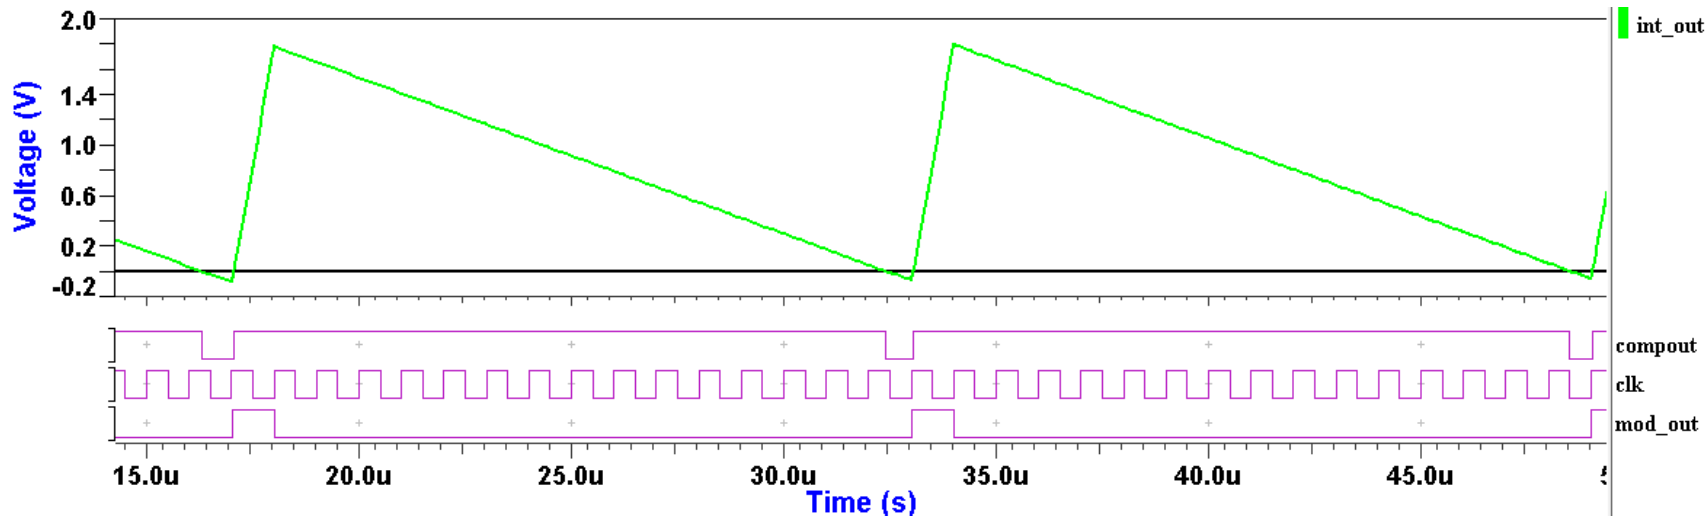
\includegraphics[width=\columnwidth]{images/sigma_delta_timing.png}

    Je nach $V_{\rm in}$ ergibt sich ein anderer DutyCycle $\frac{n}{N}$\\
    (mod out). Für $V_{\rm refn} = - V_{\rm refp}$ gilt die aufgeführte Tabelle. 
\end{minipage}
\hfill
\begin{minipage}[c]{0.38\columnwidth}
    \renewcommand{\arraystretch}{1.3}
    \begin{tabular}{c | c}
        $\bf{V_{\rm in}}$               & \textbf{Duty Cycle} $\bf{\frac{n}{N}}$ \\
        \midrule
        $0 \, \volt$                    & $\frac{1}{2}$ \\
        $\frac{1}{2} \, V_{\rm refn}$   & $\frac{1}{4}$ \\
        $\frac{7}{8} \, V_{\rm refn}$   & $\frac{1}{16}$ \\
        $\frac{1}{10} \, V_{\rm refp}$  & $\frac{11}{20}$ \\
        $0.02 \cdot \, V_{\rm refp}$    & $\frac{51}{100}$
    \end{tabular}
    \renewcommand{\arraystretch}{1}
\end{minipage}


\subsubsection*{Fazit DC-Eingangssignale}

\begin{itemize}
    \item DC-Eingangssignale erzeugen \textbf{repetitive Sequenzen} mit hohen Frequenz-Anteilen
    \item Ist $V_{\rm in}$ nahe bei Bruchteil von $V_{\rm ref}$ entstehen \textbf{lange repetitive Sequenzen} mit tiefen Frequenz-Anteilen
    \item \textbf{Lange repetitive Sequenzen können nicht von Signal unterschieden werden\\
        \textrightarrow\ Pattern Noise}
\end{itemize}
        

\subsubsection{AC-Eingangssignale}

AC-Eingangssignale können durch Mittelwertbildung (z.B. mit Tiefpassfilter mit entsprechend hoch dimensinierter Zeitkonstante) 
des Signals $V_{\rm int}$ rekonstruiert werden.


\subsection{Modellierung Sigma-Delta-Modulator im Frequenzbereich}

\begin{minipage}[c]{0.4\columnwidth}
    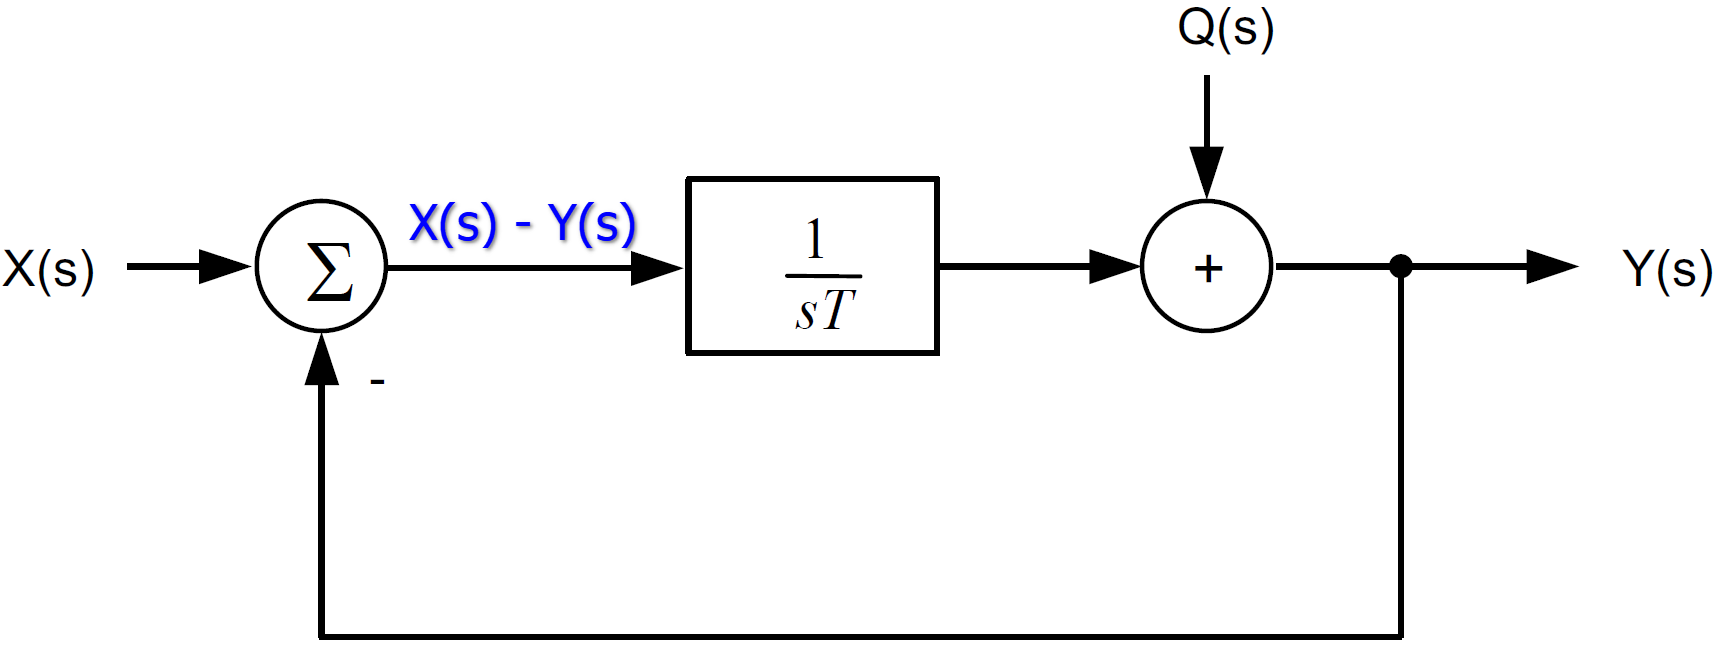
\includegraphics[width=\columnwidth]{images/sigma-delta-modulator_frequenzbereich.png}
\end{minipage}
\hfill
\begin{minipage}[c]{0.58\columnwidth}

    \begin{tabular}{ll}
        $Q(s)$          & Quantisierungsrauschen \\
        $A_{\rm ADC}$   & Verstärkungsfaktor ADC ($=1$) \\
        $A_{\rm DAC}$   & Verstärkungsfaktor DAC ($=1$) 
    \end{tabular}
\end{minipage}


\subsubsection{Übertragungsfunktionen Sigma-Delta Modulator}

\begin{minipage}[t]{0.48\columnwidth}
    \begin{center}
        \myul{Signal-Übertragungsfunktion $H_s(s)$}
        (Quantisierungsrauschen $Q(s) = 0$)
    \end{center}
    $$ Y(s) = [X(s) - Y(s)] \cdot\frac{1}{s \cdot T} $$
    $$ \boxed{ H_s(s) = \frac{Y(s)}{X(s)} = \frac{1}{1 + s \cdot T} \quad \text{(Tiefpass)}} $$
\end{minipage}
\hfill
\begin{minipage}[t]{0.48\columnwidth}
    \begin{center}
        \myul{Noise-Übertragungsfunktion $H_n(s)$}
        (Eingangssignal $X(s) = 0$)
    \end{center}
    $$ Y(s) = - Y(s) \cdot\frac{1}{s \cdot T} + Q(s) $$
    $$ \boxed{ H_n(s) = \frac{Y(s)}{Q(s)} = \frac{s \cdot T}{1 + s \cdot T} \quad \text{(Hochpass)}} $$
\end{minipage}

% gutes Bild für Noise-Übertragungsfunktion bzw. Noise-Shaping aber ka wohin damit
% 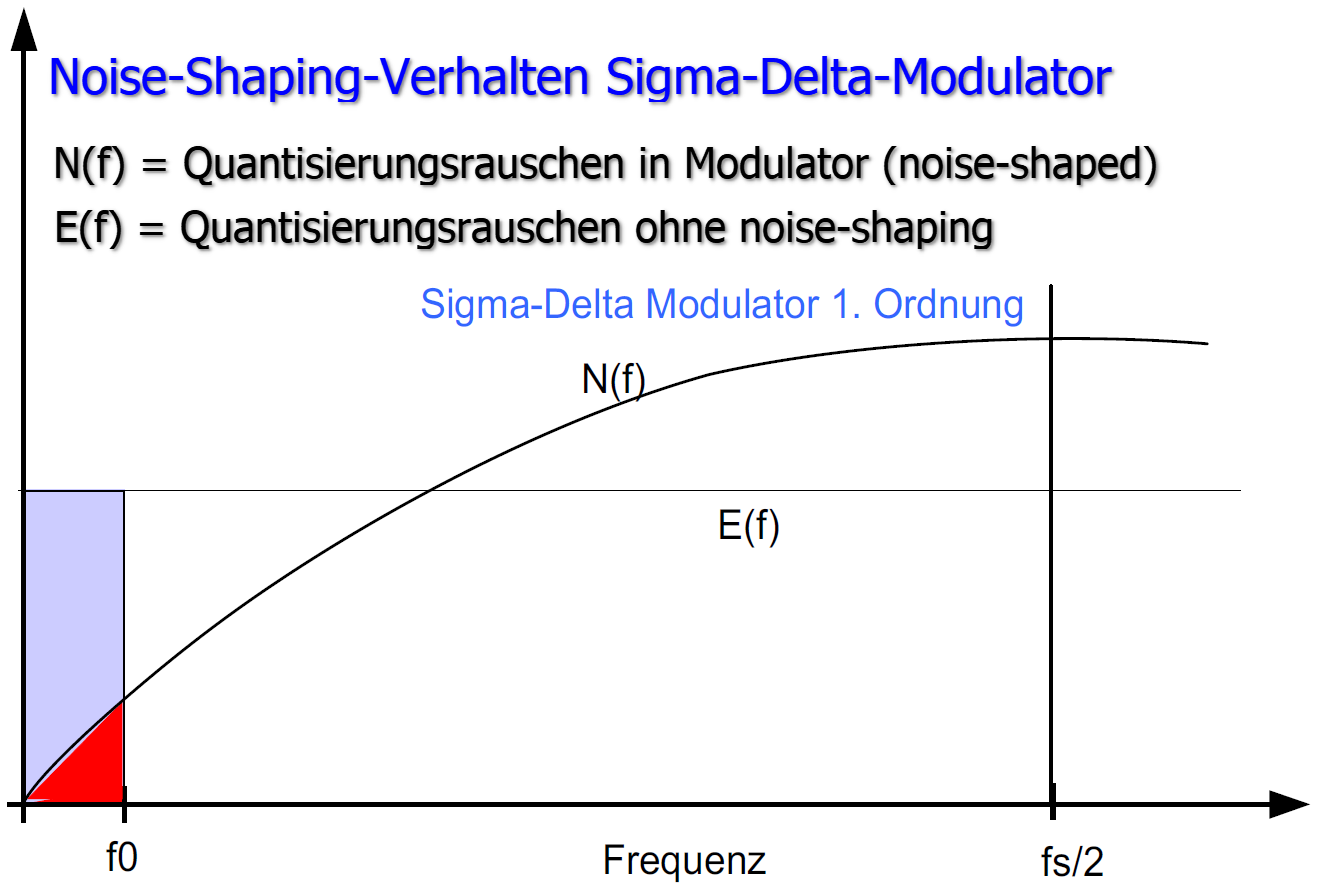
\includegraphics[width=\columnwidth]{images/noise_shaping_sigma_delta.png} 


\subsection{Oversampling / Signal-Rausch-Abstand (SNR)}

$$ \boxed{ \text{Rauschleistung} = \text{Rauschleistungsdichte} * \text{Bandbreite} = \frac{q^2}{12} = \text{konstant}} $$

\begin{itemize}
    \item Oversampling verteilt Quantisierungsrauschen über grösseren Frequenzbereich
    \item Da die Rauschleistung konstant ist, wird die Rauschleistungsdichte (also die 'Amplitude' des Rauschens) kleiner
    \item Ein Digitalfilter reduziert die Bandbreite des ADCs weiter
\end{itemize}

\begin{minipage}[c]{0.48\columnwidth}
    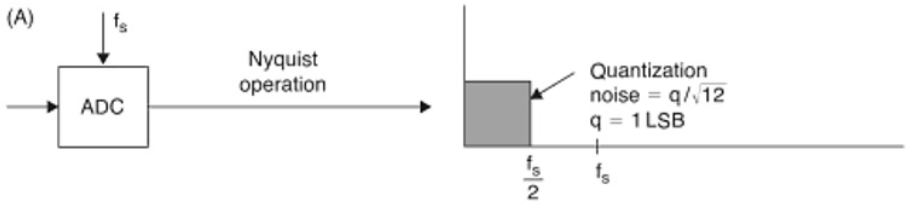
\includegraphics[width=\columnwidth]{images/rauschen_ohne_oversampling.png}
\end{minipage}
\hfill
\begin{minipage}[c]{0.48\columnwidth}
    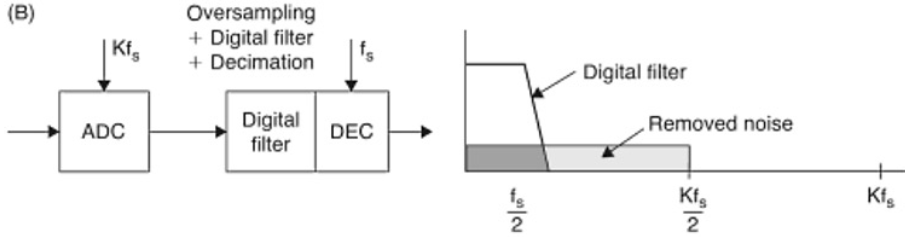
\includegraphics[width=\columnwidth]{images/rauschen_mit_oversampling.png}
\end{minipage}


\subsubsection{Noise-Shaping}

\begin{minipage}[c]{0.48\columnwidth}
    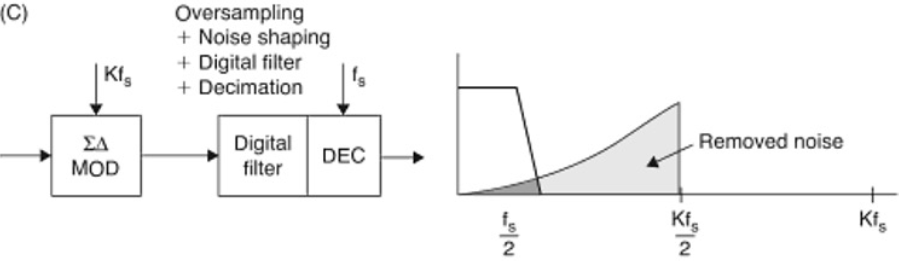
\includegraphics[width=\columnwidth]{images/rauschen_mit_oversampling_und_noise_shaping.png}
\end{minipage}
\hfill
\begin{minipage}[c]{0.48\columnwidth}
    \begin{itemize}
        \item Nicht nur Oversampling und Rauschen gleichmässig verteilen, sondern Rauschleistungsdichte 'formen'
        \item \textbf{Nur bei Sigma-Delta-Wandlern möglich}
    \end{itemize}
\end{minipage}


\subsection{Sigma-Delta-Wandler 2. Ordnung}

\begin{minipage}[c]{0.48\columnwidth}
    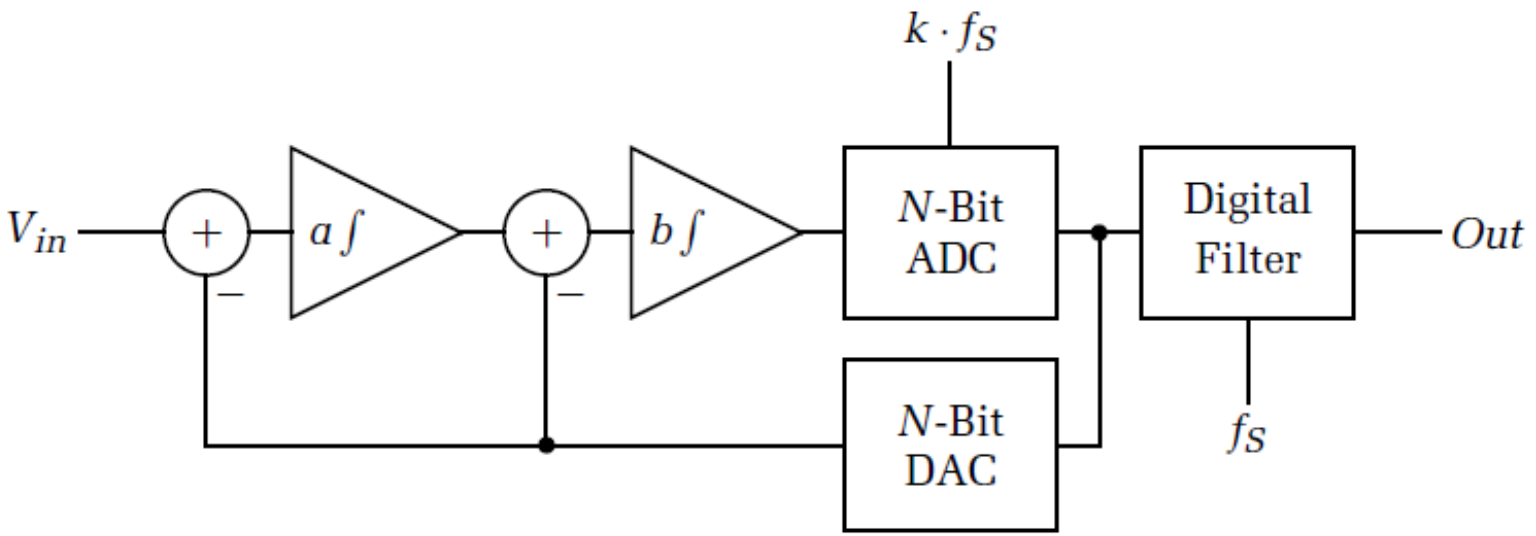
\includegraphics[width=\columnwidth]{images/sigma-delta-wandler_ordnung_2.png}
\end{minipage}
\hfill
\begin{minipage}[c]{0.5\columnwidth}
    $$ \boxed{ \text{SNR} \approx 10 \cdot \log_{10} \Bigl( \frac{3}{2} \cdot \frac{2 M + 1}{\pi^{2M}} \cdot \text{OSR}^{2M+1} \Bigr) } $$
    \begin{tabular}{ll}
        OSR & Oversampling-Rate \\
        $M$ & Ordnung des Modulators
    \end{tabular}
\end{minipage}

\begin{itemize}
    \item Ordnung $M = 2$ \textrightarrow\ 2 Integratoren
    \item Quantisierungsrauschen $Q(s)$ wird mit Hochpass 2. Ordnung gefiltert
    \item Je höher Ordnung $M$, desto stärker das Noise-Shaping ($6 \, \deci \bel$ pro Ordnung und Oktave)
    \item Je höher Oversampling (OSR), desto höher SNR ($3 \, \deci \bel$ Oktave)
\end{itemize}

